\begin{figure}
    \centering
    \subfloat[Step 1]{{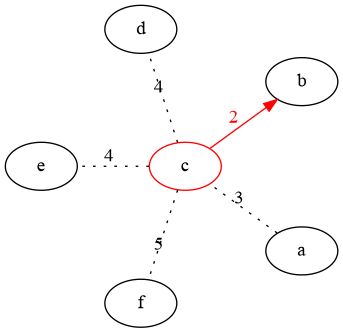
\includegraphics[width=6cm]{forest-example-1.png} }}
    \vspace{0.6cm}
    \subfloat[Step 2]{{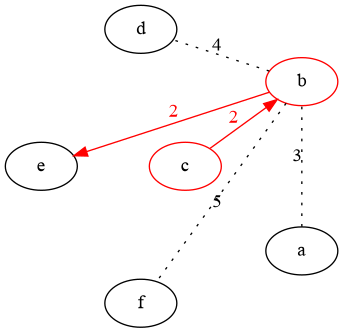
\includegraphics[width=6cm]{forest-example-2.png} }}
    \vspace{0.6cm}
    \subfloat[Step 3]{{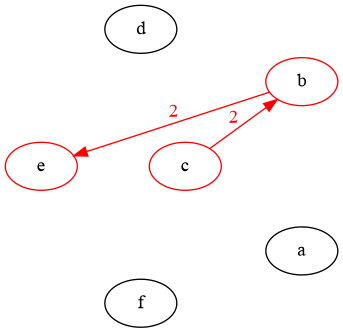
\includegraphics[width=6cm]{forest-example-3.png} }}
    \vspace{0.6cm}
    \subfloat[Step 4]{{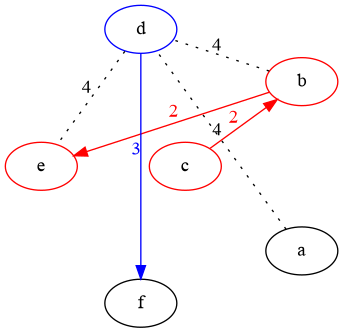
\includegraphics[width=6cm]{forest-example-4.png} }}
    \vspace{0.6cm}
    \subfloat[Step 5]{{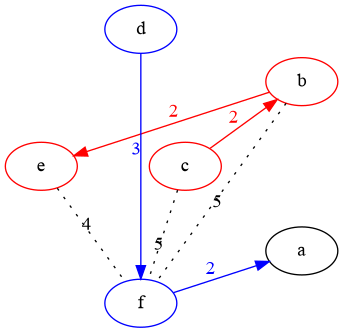
\includegraphics[width=6cm]{forest-example-5.png} }}
    \vspace{0.6cm}
    \subfloat[Step 6]{{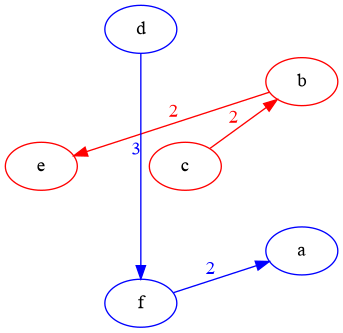
\includegraphics[width=6cm]{forest-example-6.png} }}
    \caption{Forest Building Algorithm}\label{fig:forest_partitioning}
\end{figure}